\documentclass[spec, och, otchet, hidelinks]{SCWorks}
% параметр - тип обучения - одно из значений:
%    spec     - специальность
%    bachelor - бакалавриат (по умолчанию)
%    master   - магистратура
% параметр - форма обучения - одно из значений:
%    och   - очное (по умолчанию)
%    zaoch - заочное
% параметр - тип работы - одно из значений:
%    otchet
%    referat    - реферат
%    coursework - курсовая работа (по умолчанию)
%    diploma    - дипломная работа
%    pract      - отчет по практике
%    pract      - отчет о научно-исследовательской работе
%    autoref    - автореферат выпускной работы
%    assignment - задание на выпускную квалификационную работу
%    review     - отзыв руководителя
%    critique   - рецензия на выпускную работу
% параметр - включение шрифта
%    times    - включение шрифта Times New Roman (если установлен)
%               по умолчанию выключен
\usepackage[T2A]{fontenc}
\usepackage[utf8]{inputenc}
\usepackage{graphicx}

\usepackage[sort,compress]{cite}
\usepackage{amsmath}
\usepackage{amssymb}
\usepackage{amsthm}
\usepackage{fancyvrb}
\usepackage{longtable}
\usepackage{array}
\usepackage[english,russian]{babel}
\usepackage{minted}
% Используется автором репозитория
%\usemintedstyle{xcode}
% Этот пакет включает в себя аналогичный Times New Roman шрифт.
% Необходим для успешной компиляции для UNIX-систем ввиду отсутствия TNR в нем.
% Можно использовать и для Windows.
\usepackage{tempora}


\usepackage[colorlinks=false]{hyperref}

\graphicspath{{figures/}}

\newcommand{\eqdef}{\stackrel {\rm def}{=}}

\usepackage{stackengine}
\newcommand\xrowht[2][0]{\addstackgap[.5\dimexpr#2\relax]{\vphantom{#1}}}

\newtheorem{lem}{Лемма}

% % При использовании biblatex вместо bibtex
%\usepackage[style=gost-numeric]{biblatex}
%\addbibresource{thesis.bib}

\begin{document}

% Кафедра (в родительном падеже)
\chair{математической кибернетики и компьютерных наук}

% Тема работы
\title{Регистры}

% Курс
\course{3}

% Группа
\group{331}

% Факультет (в родительном падеже) (по умолчанию "факультета КНиИТ")
%\department{факультета КНиИТ}

% Специальность/направление код - наименование
%\napravlenie{02.03.02 "--- Фундаментальная информатика и информационные технологии}
%\napravlenie{02.03.01 "--- Математическое обеспечение и администрирование информационных систем}
%\napravlenie{09.03.01 "--- Информатика и вычислительная техника}
%\napravlenie{09.03.04 "--- Программная инженерия}
\napravlenie{10.05.01 "--- Компьютерная безопасность}

% Для студентки. Для работы студента следующая команда не нужна.
%\studenttitle{Студентки}

% Фамилия, имя, отчество в родительном падеже
\author{Бородина Артёма Горовича}

% Заведующий кафедрой
\chtitle{доцент, к.\,ф.-м.\,н.} % степень, звание
\chname{С.\,В.\,Миронов}

%Научный руководитель (для реферата преподаватель проверяющий работу)
\satitle{аспирант}%, к.\,ф.-м.\,н.} %должность, степень, звание
\saname{А.\,А.\,Мартышкин}

% Руководитель практики от организации (только для практики,
% для остальных типов работ не используется)
\patitle{к.\,ф.-м.\,н., доцент}
\paname{Д.\,Ю.\,Петров}

% Семестр (только для практики, для остальных
% типов работ не используется)
\term{2}

% Наименование практики (только для практики, для остальных
% типов работ не используется)
\practtype{учебная}

% Продолжительность практики (количество недель) (только для практики,
% для остальных типов работ не используется)
\duration{2}

% Даты начала и окончания практики (только для практики, для остальных
% типов работ не используется)
\practStart{01.07.2016}
\practFinish{14.07.2016}

% Год выполнения отчета
\date{2022}

\maketitle

% Включение нумерации рисунков, формул и таблиц по разделам
% (по умолчанию - нумерация сквозная)
% (допускается оба вида нумерации)
%\secNumbering


\tableofcontents

% Раздел "Обозначения и сокращения". Может отсутствовать в работе
% \abbreviations
% \begin{description}
%     \item ... "--- ...
%     \item ... "--- ...
% \end{description}

% Раздел "Определения". Может отсутствовать в работе
%\definitions

% Раздел "Определения, обозначения и сокращения". Может отсутствовать в работе.
% Если присутствует, то заменяет собой разделы "Обозначения и сокращения" и "Определения"
%\defabbr


% Раздел "Введение"

\intro

\par Целью данной работы служит ознакомление с устройством и функционированием регистров и регистровой памяти, а также испытание интегрального 
универсального регистра сдвига.

\newpage

\section*{Задание 1.}
\addcontentsline{toc}{section}{Задание 1}

\par Запустить лабораторный комплекс Labworks и среду МS10. Открыть файл \textbf{33.4.ms10}, размещенный в папке \textbf{Circuit Design Suitе 10.0} 
среды МS10, или собрать на рабочем
поле среды MS10 схему для испытания \textit{универсального регистра сдвига} и установить в диалоговых окнах компонентов их параметры или режимы работы.
\textbf{Скопировать} схему в отчет.

\newpage

\section*{Задание 2.}
\addcontentsline{toc}{section}{Задание 2}

\textbf{Составить} план исследования параллельного регистра сдвига, заполнив ячейки памяти генератора слова \textbf{XWG1} на основе правил 
функционирования регистра \textbf{74НС194\_4V}, отраженных в табл. 1.

\begin{figure}[h]
	\center{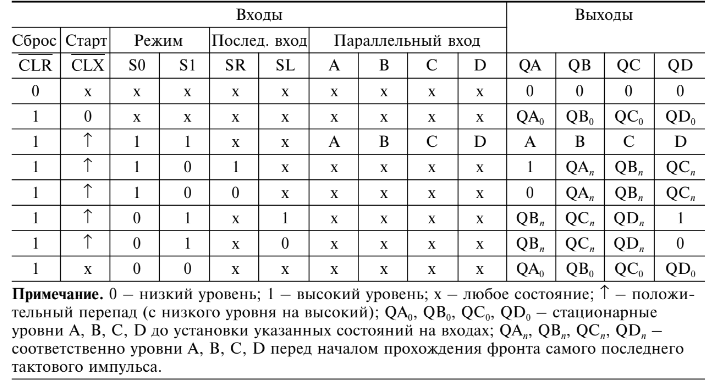
\includegraphics{table.png}}
	\caption{Схема шифратора.}
\end{figure}


\conclusion

\par В ходе данной лабораторной работы мы ознакомились с основными характеристиками интегральных 
преобразователей кодов (дешифратора, шифратора, демультиплексора и мультиплексора) 
и испытали эти устройства путём составления диаграмм их входных и выходных сигналов.

\end{document}